% !TeX root = Thesis.tex

\begin{figure}[!htbp]
  \centering
  \begin{tikzpicture}[level distance=1cm,
    level 1/.style={sibling distance=9cm},
    level 2/.style={sibling distance=5cm}]
    \node {n=3}
      child { node {$H$ exists}
        child { node {$\underset{\raisebox{-0.8em}{3}}{\text{LP integral solution}}$} }
        child { node {$\underset{\raisebox{-0.8em}{0}}{\text{LP fractional solution}}$} }
      }
      child { node {$H$ does not exist}
        child { node {$\underset{\raisebox{-0.8em}{1}}{\text{LP infeasible}}$} }
        child { node {$\underset{\raisebox{-0.8em}{0}}{\text{LP fractional solution}}$} }
      };
  \end{tikzpicture}

  \begin{tikzpicture}[level distance=1cm,
    level 1/.style={sibling distance=9cm},
    level 2/.style={sibling distance=5cm}]
    \node {n=4}
      child { node {$H$ exists}
        child { node {$\underset{\raisebox{-0.8em}{6}}{\text{LP integral solution}}$} }
        child { node {$\underset{\raisebox{-0.8em}{0}}{\text{LP fractional solution}}$} }
      }
      child { node {$H$ does not exist}
        child { node {$\underset{\raisebox{-0.8em}{5}}{\text{LP infeasible}}$} }
        child { node {$\underset{\raisebox{-0.8em}{0}}{\text{LP fractional solution}}$} }
      };
  \end{tikzpicture}

  \begin{tikzpicture}[level distance=1cm,
    level 1/.style={sibling distance=9cm},
    level 2/.style={sibling distance=5cm}]
    \node {n=5}
      child { node {$H$ exists}
        child { node {$\underset{\raisebox{-0.8em}{9}}{\text{LP integral solution}}$} }
        child { node {$\underset{\raisebox{-0.8em}{2}}{\text{LP fractional solution}}$} }
      }
      child { node {$H$ does not exist}
        child { node {$\underset{\raisebox{-0.8em}{20}}{\text{LP infeasible}}$} }
        child { node {$\underset{\raisebox{-0.8em}{3}}{\text{LP fractional solution}}$} }
      };
  \end{tikzpicture}

  \begin{tikzpicture}[level distance=1cm,
    level 1/.style={sibling distance=9cm},
    level 2/.style={sibling distance=5cm}]
    \node {n=6}
      child { node {$H$ exists}
        child { node {$\underset{\raisebox{-0.8em}{15}}{\text{LP integral solution}}$} }
        child { node {$\underset{\raisebox{-0.8em}{13}}{\text{LP fractional solution}}$} }
      }
      child { node {$H$ does not exist}
        child { node {$\underset{\raisebox{-0.8em}{107}}{\text{LP infeasible}}$} }
        child { node {$\underset{\raisebox{-0.8em}{21}}{\text{LP fractional solution}}$} }
      };
  \end{tikzpicture}

  \begin{tikzpicture}[level distance=1cm,
    level 1/.style={sibling distance=9cm},
    level 2/.style={sibling distance=5cm}]
    \node {n=7}
      child { node {$H$ exists}
        child { node {$\underset{\raisebox{-0.8em}{25}}{\text{LP integral solution}}$} }
        child { node {$\underset{\raisebox{-0.8em}{52}}{\text{LP fractional solution}}$} }
      }
      child { node {$H$ does not exist}
        child { node {$\underset{\raisebox{-0.8em}{767}}{\text{LP infeasible}}$} }
        child { node {$\underset{\raisebox{-0.8em}{200}}{\text{LP fractional solution}}$} }
      };
  \end{tikzpicture}

  \begin{tikzpicture}[level distance=1cm,
    level 1/.style={sibling distance=9cm},
    level 2/.style={sibling distance=5cm}]
    \node {n=8}
      child { node {$H$ exists}
        child { node {$\underset{\raisebox{-0.8em}{47}}{\text{LP integral solution}}$} }
        child { node {$\underset{\raisebox{-0.8em}{260}}{\text{LP fractional solution}}$} }
      }
      child { node {$H$ does not exist}
        child { node {$\underset{\raisebox{-0.8em}{9380}}{\text{LP infeasible}}$} }
        child { node {$\underset{\raisebox{-0.8em}{2659}}{\text{LP fractional solution}}$} }
      };
  \end{tikzpicture}

  \caption{LP outcomes for different values of $n$ on base linear program.} 
  \footnotemark 
  \label{fig::linear_program_diagram} 
\end{figure}

\footnotetext{
The LP integral solution sequence $2, 3, 6, 10, 17, 29, 51, \dots$ seems to be given by \href{https://oeis.org/A285665}{A285665}.
}